\section{Experimentación}

\subsection{Variación en la cantidad de nodos}
En esta experimentación, generamos grafos de la siguiente manera: \\
\begin{itemize}
\item n fue variando entre 10, 100, 200, 300, 400 y 500.
\item m siempre mantuvo la proporción m = $\frac{n*(n-1)}{4}$
\item los costos de nafta fueron elegidos de manera aleatoria en el rango [1,100]
\item los largos de las rutas en litros fueron tomados de manera aleatoria en el rango [1,60]
\end{itemize}

La idea es ver como se comportan los distintos algoritmos, cuando vamos teniendo un grafo denso cada vez más grande. Es importante tener en cuenta que ambas versiones de Dijkstra y Bellman-Ford fueron corridos n veces (ya que el output del programa tiene todas las distancias posibles) mientras que Floyd se corre una única vez. \\
Los resultados obtenidos fueron los siguientes:
\begin{figure}[H]
   \begin{minipage}{0.5\textwidth}
     \centering
     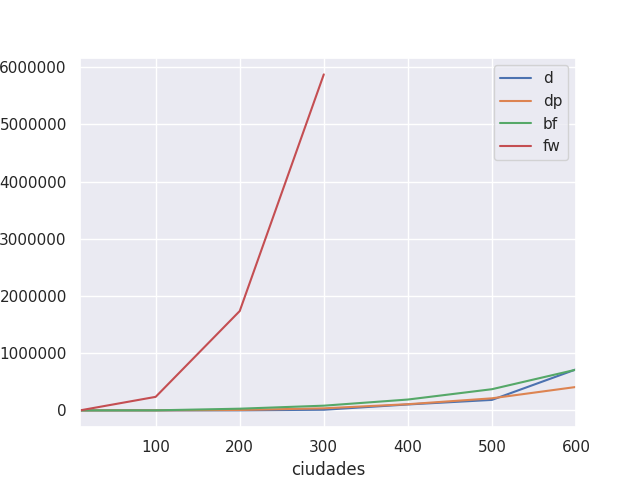
\includegraphics[width=1\linewidth]{img/exp1_2.png}
     \caption{Comparación del problema con los 4 algoritmos}
   \end{minipage}\hfill
   \begin{minipage}{0.5\textwidth}
     \centering
     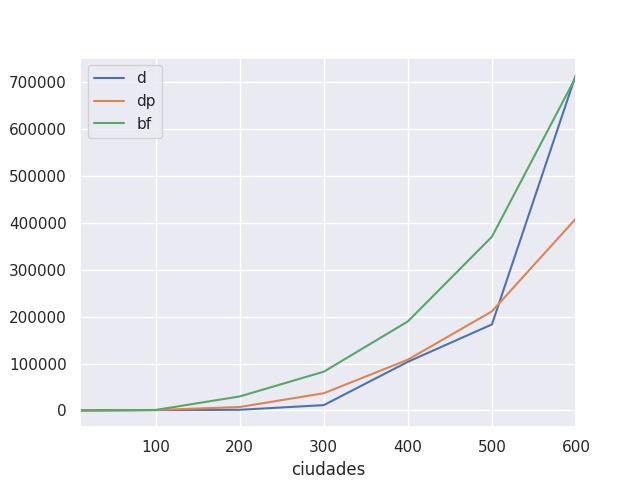
\includegraphics[width=1\linewidth]{img/exp1_1.png}
     \caption{Comparación del problema quitando el algoritmo de Floyd}
   \end{minipage}
\end{figure}

Como podemos observar, el algoritmo de Floyd crece de manera mucho más acelerada que los otros algoritmos, a tal punto que no pudo ser corrido para los casos más grandes. Esto puede deberse a que el grafo modificado que usamos para resolver el problema tiene 61*n nodos, por lo que la matríz que debe resolver Floyd resulta muy grande. De esta manera, está calculando las distancias mínimas tomando como origen a cualquier estado (cantidad de litros iniciales) de una ciudad, cuando sólamente nos importa tomar el estado del tanque vacío como origen. Esto no afecta tan marcadamente a los otros algoritmos, ya que únicamente los corremos con dicho estado como origen. \\
\indent En este caso, sabemos que m=$\mathcal{O}(n^{2})$, por lo que las complejidades de cada algoritmo corrido n veces son:
\begin{itemize}
\item Dijkstra: $\mathcal{O}(n^{3})$
\item Dijkstra con cola de prioridad: $\mathcal{O}(n^{3}*lgn)$
\item Bellman-Ford: $\mathcal{O}(n^{4})$
\item Floyd: $\mathcal{O}(n^{3})$
\end{itemize}

Como se ve en el gráfico, todas las curvas tienen un crecimiento polinomial, como se esperaba. Lo que quizas es mas inusual, es el comportamiento del algoritmo de dijkstra sin cola de prioridad. En estos casos, se esperaría que tenga una mejor performance que los demás, pero vemos que tiene un crecimiento considerablemente más acelerado. Esto probablemente se deba a que, aunque m=$\mathcal{O}(n^{2})$, en el grafo modificado la constante oculta sea lo suficientemente pequeña como para que $n^{2}$ sea considerablemente peor a m en la práctica.

\subsection{Variación en la proporción de aristas}
En esta experimentación, generamos grafos de la siguiente manera: \\
\begin{itemize}
\item n fue fijado en 100.
\item m fue variando entre 10, 100, 500, 1000, 1500, 2000, 3000, 4000
\item los costos de nafta fueron elegidos de manera aleatoria en el rango [1,100]
\item los largos de las rutas en litros fueron tomados de manera aleatoria en el rango [1,60]
\end{itemize}

En este experimento analizamos que sucede si, dado un conjunto fijo de ciudades, vamos construyendo nuevas rutas. Al igual que en el experimento anterior, todos los algoritmos salvo el de Floyd fueron corridos n=100 veces. \\
Veamos los resultados:
\begin{figure}[H]
   \begin{minipage}{0.5\textwidth}
     \centering
     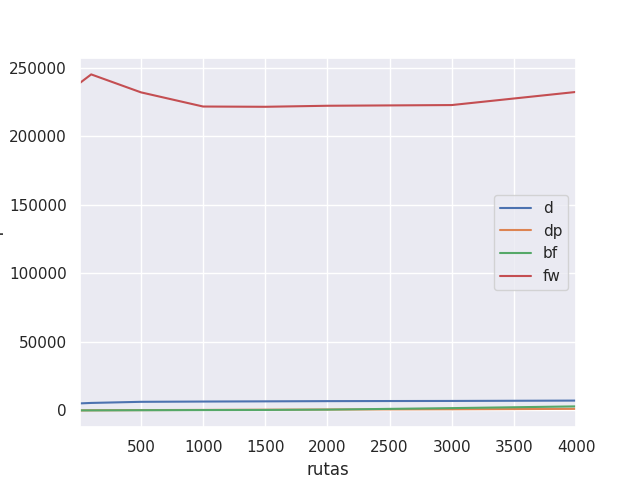
\includegraphics[width=1\linewidth]{img/exp2_2.png}
     \caption{Comparación del problema con los 4 algoritmos}
   \end{minipage}\hfill
   \begin{minipage}{0.5\textwidth}
     \centering
     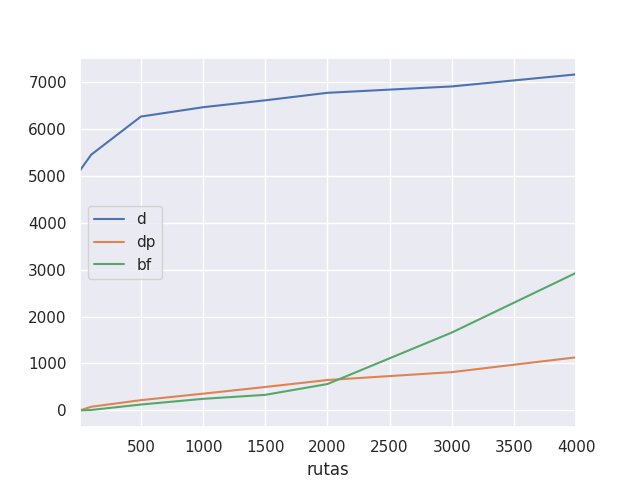
\includegraphics[width=1\linewidth]{img/exp2_1.png}
     \caption{Comparación del problema quitando el algoritmo de Floyd}
   \end{minipage}
\end{figure}

Nuevamente, el algoritmo de Floyd fue mucho más lento que los demás. Sin embargo, podemos ver que en este caso el tiempo de computo de Floyd se mantiene constante. Esto era de esperarse, pues la complejidad del mismo depende únicamente de n, que fue fijado en 100.
En cuanto a los otros algoritmos, asumiendo que en este caso n es una constante, las complejidades teóricas en cada caso son:
\begin{itemize}
\item Dijkstra: $\mathcal{O}(1)$
\item Dijkstra con cola de prioridad: $\mathcal{O}(m)$
\item Bellman-Ford: $\mathcal{O}(m)$
\end{itemize}
Sin embargo, es importante notar que existe un $\mathcal{O}(m)$ en la complejidad del algoritmo de Dijkstra sin cola de prioridad, ya que se recorren todas las aristas. Esto explica el crecimiento de su curva en el gráfico. En cuanto a Bellman-Ford y Dijkstra con cola de prioridad, si recordamos que el m va acompañado de un n y de un log(n) respectivamente, podemos explicar por qué difieren las pendientes de sus rectas.
